% *********************************************************************
% © 2024 Jeremy Sylvestre
%
% Permission is granted to copy, distribute and/or modify this document
% under the terms of the GNU Free Documentation License, Version 1.3 or
% any later version published by the Free Software Foundation; with no
% Invariant Sections, no Front-Cover Texts, and no Back-Cover Texts. A
% copy of the license is included in the appendix entitled “GNU Free
% Documentation License” that appears in the output document of this
% PreTeXt source code. All trademarks™ are the registered® marks of
% their respective owners.
%
% *********************************************************************

\newcommand*{\xmin}{-0.25}
\newcommand*{\xmax}{3.05}
\newcommand*{\ymin}{-0.5}
\newcommand*{\ymax}{2.25}

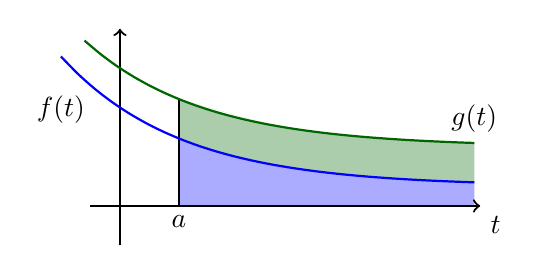
\begin{tikzpicture}[xscale=1.5]

	\fill[blue,opacity=0.33] plot[domain=0.5:3,smooth] (\x,{exp(- \x) + 0.25}) -- (3,0) -- (0.5,0) -- (0.5,0.857);
	\fill[green!40!black,opacity=0.33]
	  plot[domain=0.5:3,smooth] (\x,{exp(- \x) + 0.75})
	  -- (3,0.3)
	  plot[domain=3:0.5,smooth] (\x,{exp(- \x) + 0.25})
	  -- (0.5,1.357);

	% axes
	\draw[->,thick] (\xmin,0) -- (\xmax,0) node[below right] {$t$};
	\draw[->,thick] (0,\ymin) -- (0,\ymax);

	\draw[thin] (0.5,1.357) -- (0.5,0) node[below] {$a$};

	\draw[thick, green!40!black, domain=-0.3:3,smooth] plot (\x,{exp(-\x) + 0.75}) node[above,black] {$g(t)$};
	\draw[thick, blue, domain=3:-0.5,smooth] plot (\x,{exp(- \x) + 0.25}) node[black,yshift=-0.67cm] {$f(t)$};

\end{tikzpicture}
